%This is my super simple Real Analysis Homework template

\documentclass{article}
\usepackage[english]{babel}
\usepackage[]{amsthm} %lets us use \begin{proof}
\usepackage[]{amssymb} %gives us the character \varnothing
\usepackage{mathtools}
\usepackage{lineno}
\usepackage[ansinew]{inputenc}
\newcommand{\R}{\mathbb{R}}
\newcommand{\uproman}[1]{\uppercase\expandafter{\romannumeral#1}}
\title{Solutions Sheet}
\author{Nina Fischer and Yannick Zelle}
\date\today
%This information doesn't actually show up on your document unless you use the maketitle command below

\begin{document}
\maketitle %This command prints the title based on information entered above

%Section and subsection automatically number unless you put the asterisk next to them.


%Basically, you type whatever text you want and use the $ sign to enter "math mode".
%For fancy calligraphy letters, use \mathcal{}
%Special characters are their own commands

\section*{Exercise 1}
 

\section*{Exercise 2}


\section*{Exercise 3}
Our Implementation of exercise 3 can be seen in the attached notebook.

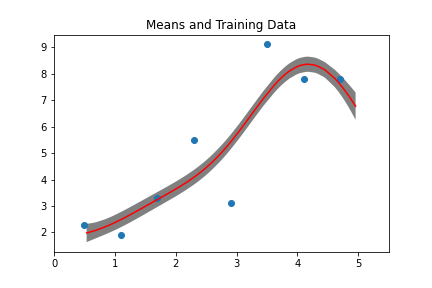
\includegraphics[width=0.75\textwidth]{EX3.png}
\section*{Exercise 4}
The Resulting Plots are :

\begin{figure}[h]
    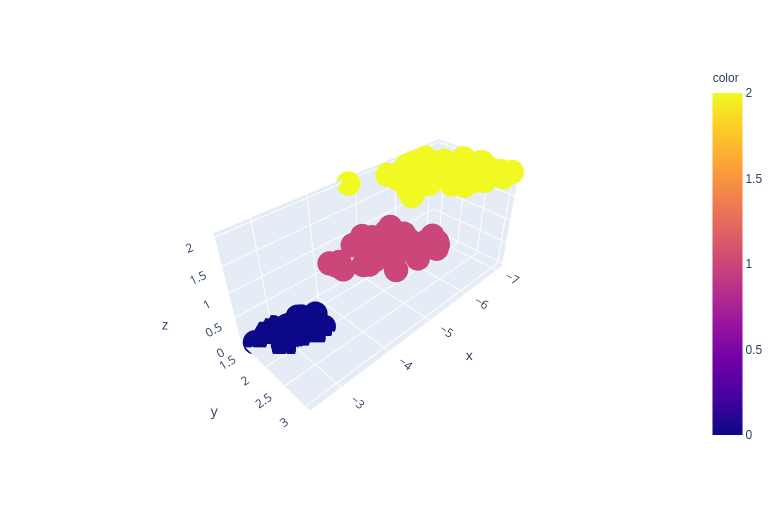
\includegraphics[width=1\textwidth]{wout_W.png}
    \caption{Without Whitening}
 \end{figure}
\newpage
\begin{figure}[h]
    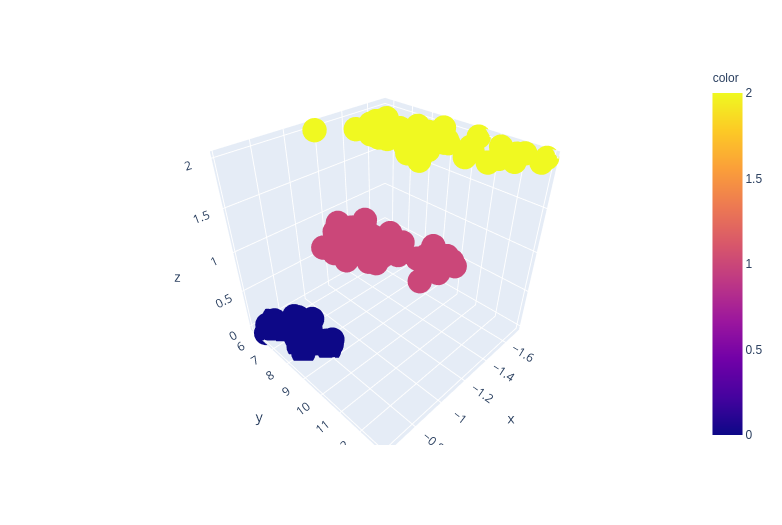
\includegraphics[width=1\textwidth]{with_w.png}
    \caption{With Whitening}
\end{figure}
For implementation details see attached notebook

\section*{Execrcise 5}
\begin{itemize}
    \item[\textbf{(a)}] 
    \begin{proof}
        
    
    \begin{align*}
        \Phi^T(a)\Phi(b)    &= a_1^2b_1^2+a_2^2+b_2^2+2a_1a_2b_1b_2+2a_1b_1+2a_2b_2+1\\
                            &= a_1^2b_1^2+ 2a_1b_1a_2b_2+a_2^2+b_2^2+2a_1b_1+2a_2b_2+1\\
                            &=(a_1b_1+a_2b_2)^2(a_1b_1+a_2b_2)+1\\
                            &=((a_1b_1+a_2b_2)^2+1)^2\\
                            &=(a^Tb+1)^2\\
                            &=k(a,b)
    \end{align*}
\end{proof} 
    \item[\textbf{(b)}] The corresponding feature space is :
    \[
    \Phi(a)= [a_1^3,a_2^3,\sqrt{3}a_1a_2^2,\sqrt{3}a_1^2a_2,\sqrt{3}a_1^2,\sqrt{6}a_1a_2,\sqrt{3}a_1,\sqrt{3}a_2^2,\sqrt{3}a_2,1]^T  
    \] 
    The feature space is ten diagonal
\item[\textbf{(c)}] The corresponding featurespace has $p^2+1$ dimensions

\end{itemize}


\end{document}
